% !TeX spellcheck = en_GB 
\section{Conclusion}
The diagonal interlocking design outperforms the straight design and existing dovetail designs,
but the standard deviation is too high to make that conclusion definitive.
All tested interlocking designs can reach between 6 and 7 \si{\mega\pascal}, which is roughly \SI{80}{\percent} of the theoretical maximum of \SI{8.6}{\mega\pascal},
but the optimal diagonal design produces the best average tensile strength.

The analytical models can be used to quickly get a rough estimate of optimal interlocking designs,
which might come in handy when considering different materials.
Performing FEM simulations of interlocking structure behaviour is time consuming and provides results which are comparable to analytical methods.

Genus interlocking shows potential for high compliance materials, because deformation isn't enough to break the interlock.
It can help with complex and slanted surfaces, because genus interlocking locks translation in each dimension, 
whereas dovetail designs allow for translation along Z.



\subsection{Applications}
While TPLA is a relatively tough and stiff material, PP is more compliant and doesn't fatigue easily.
As such PP is often used for living hinges, which consist of a single part.
Combining these materials unlocks compliant mechanism applications.
See \cref{fig:applications}.


\begin{figure}
	\setlength{\figheight}{.5\columnwidth}
	\centering
	\begin{subfigure}[B]{.35\columnwidth}
		\centering
		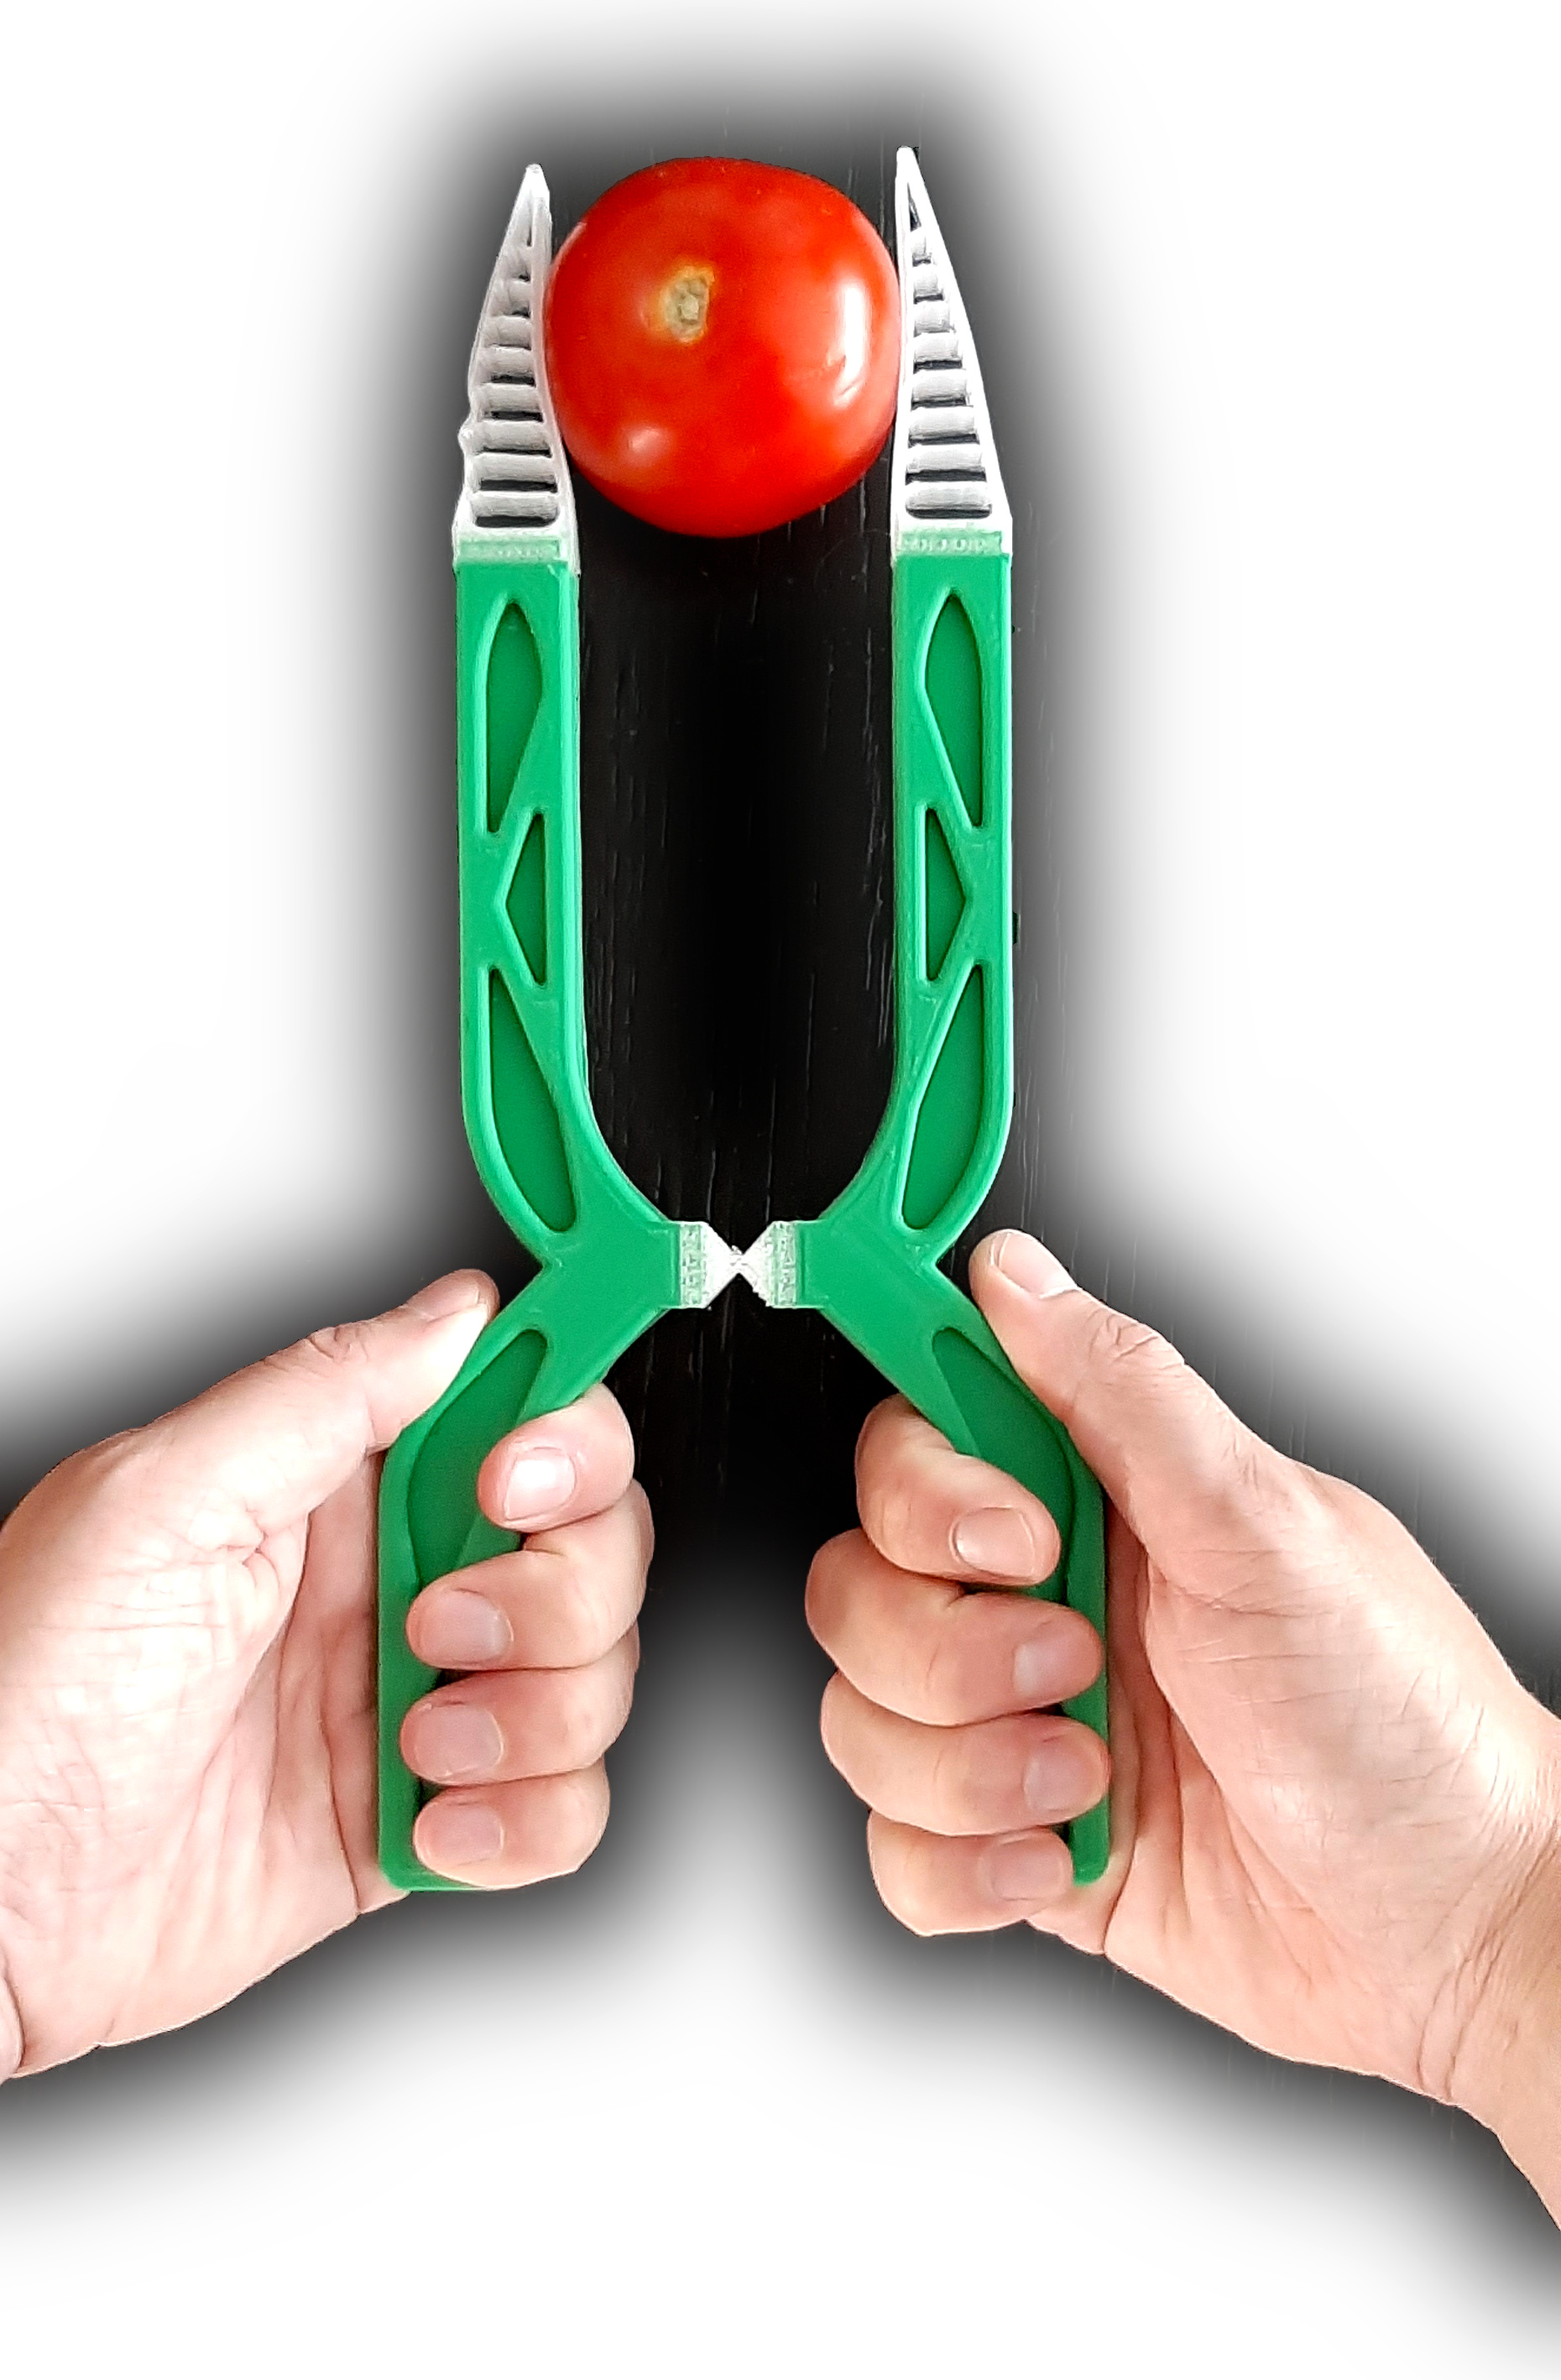
\includegraphics[height=\figheight]{sources/applications/gripper.jpg}
		\caption{Gripper}
	\end{subfigure}
	\begin{subfigure}[B]{.3\columnwidth}
		\centering
		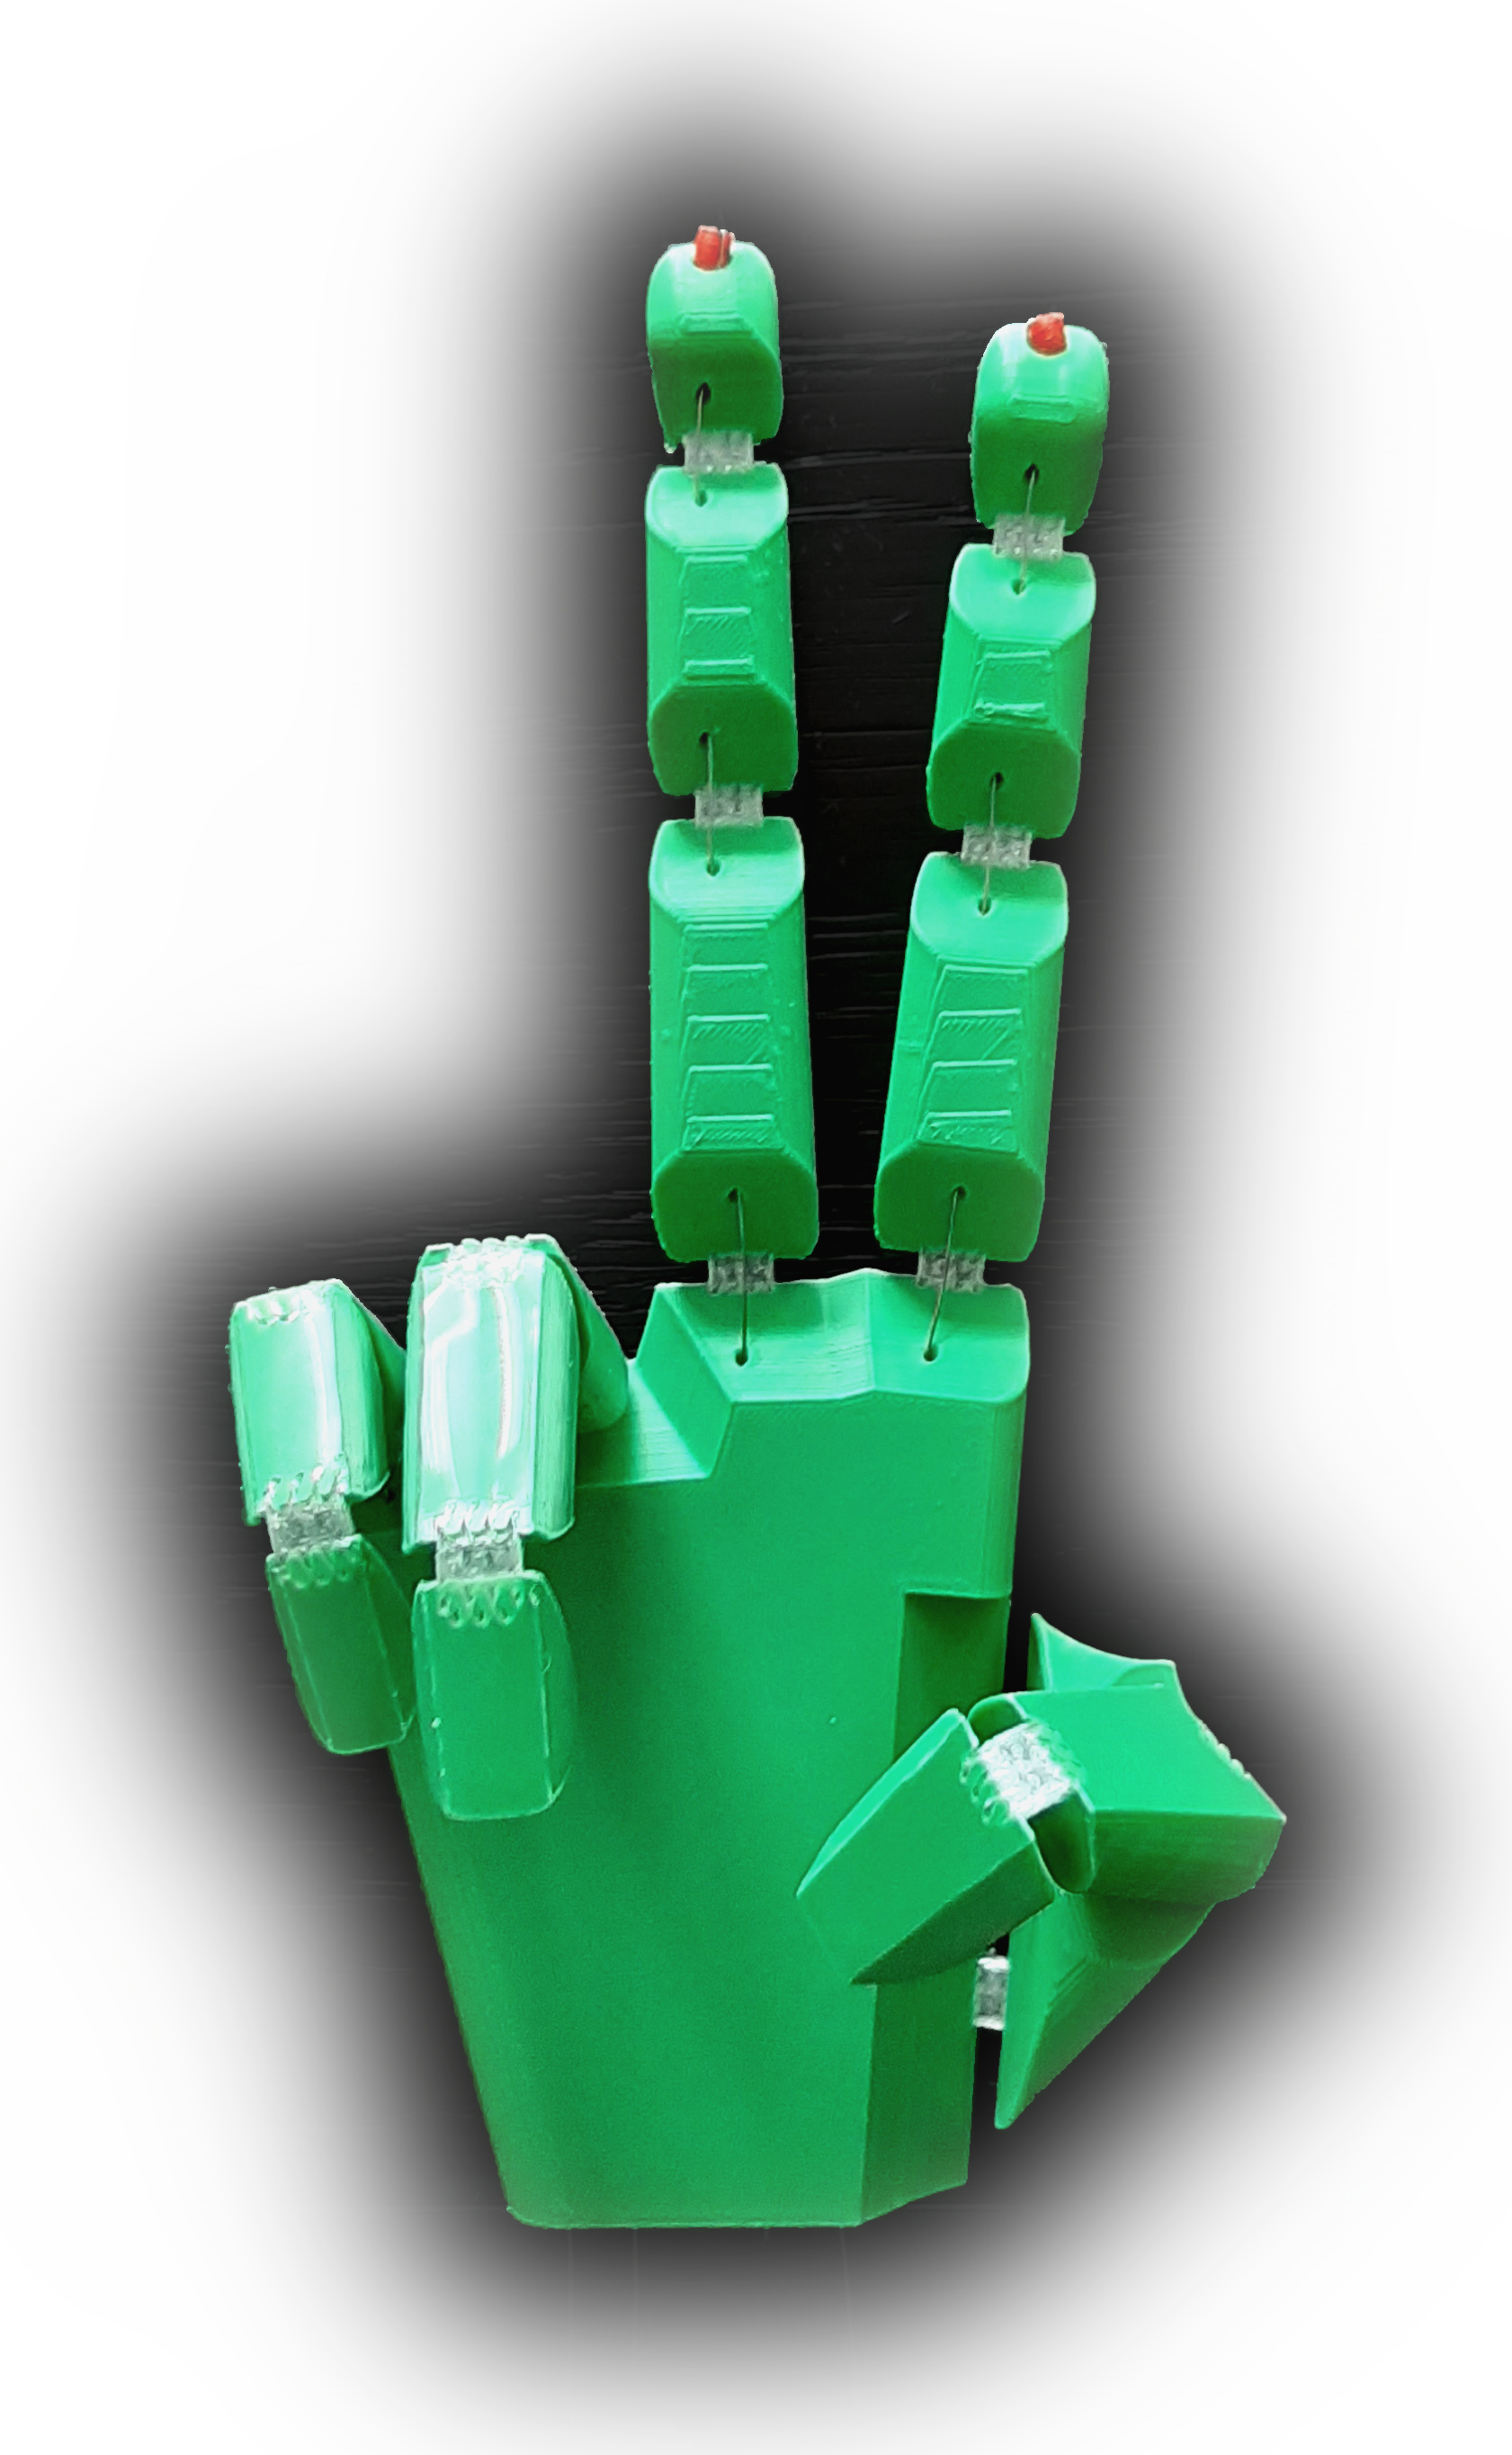
\includegraphics[height=\figheight]{sources/applications/prosthetic.jpg}
		\caption{Prosthetic}
	\end{subfigure}
	\begin{subfigure}[B]{.3\columnwidth}
		\centering
		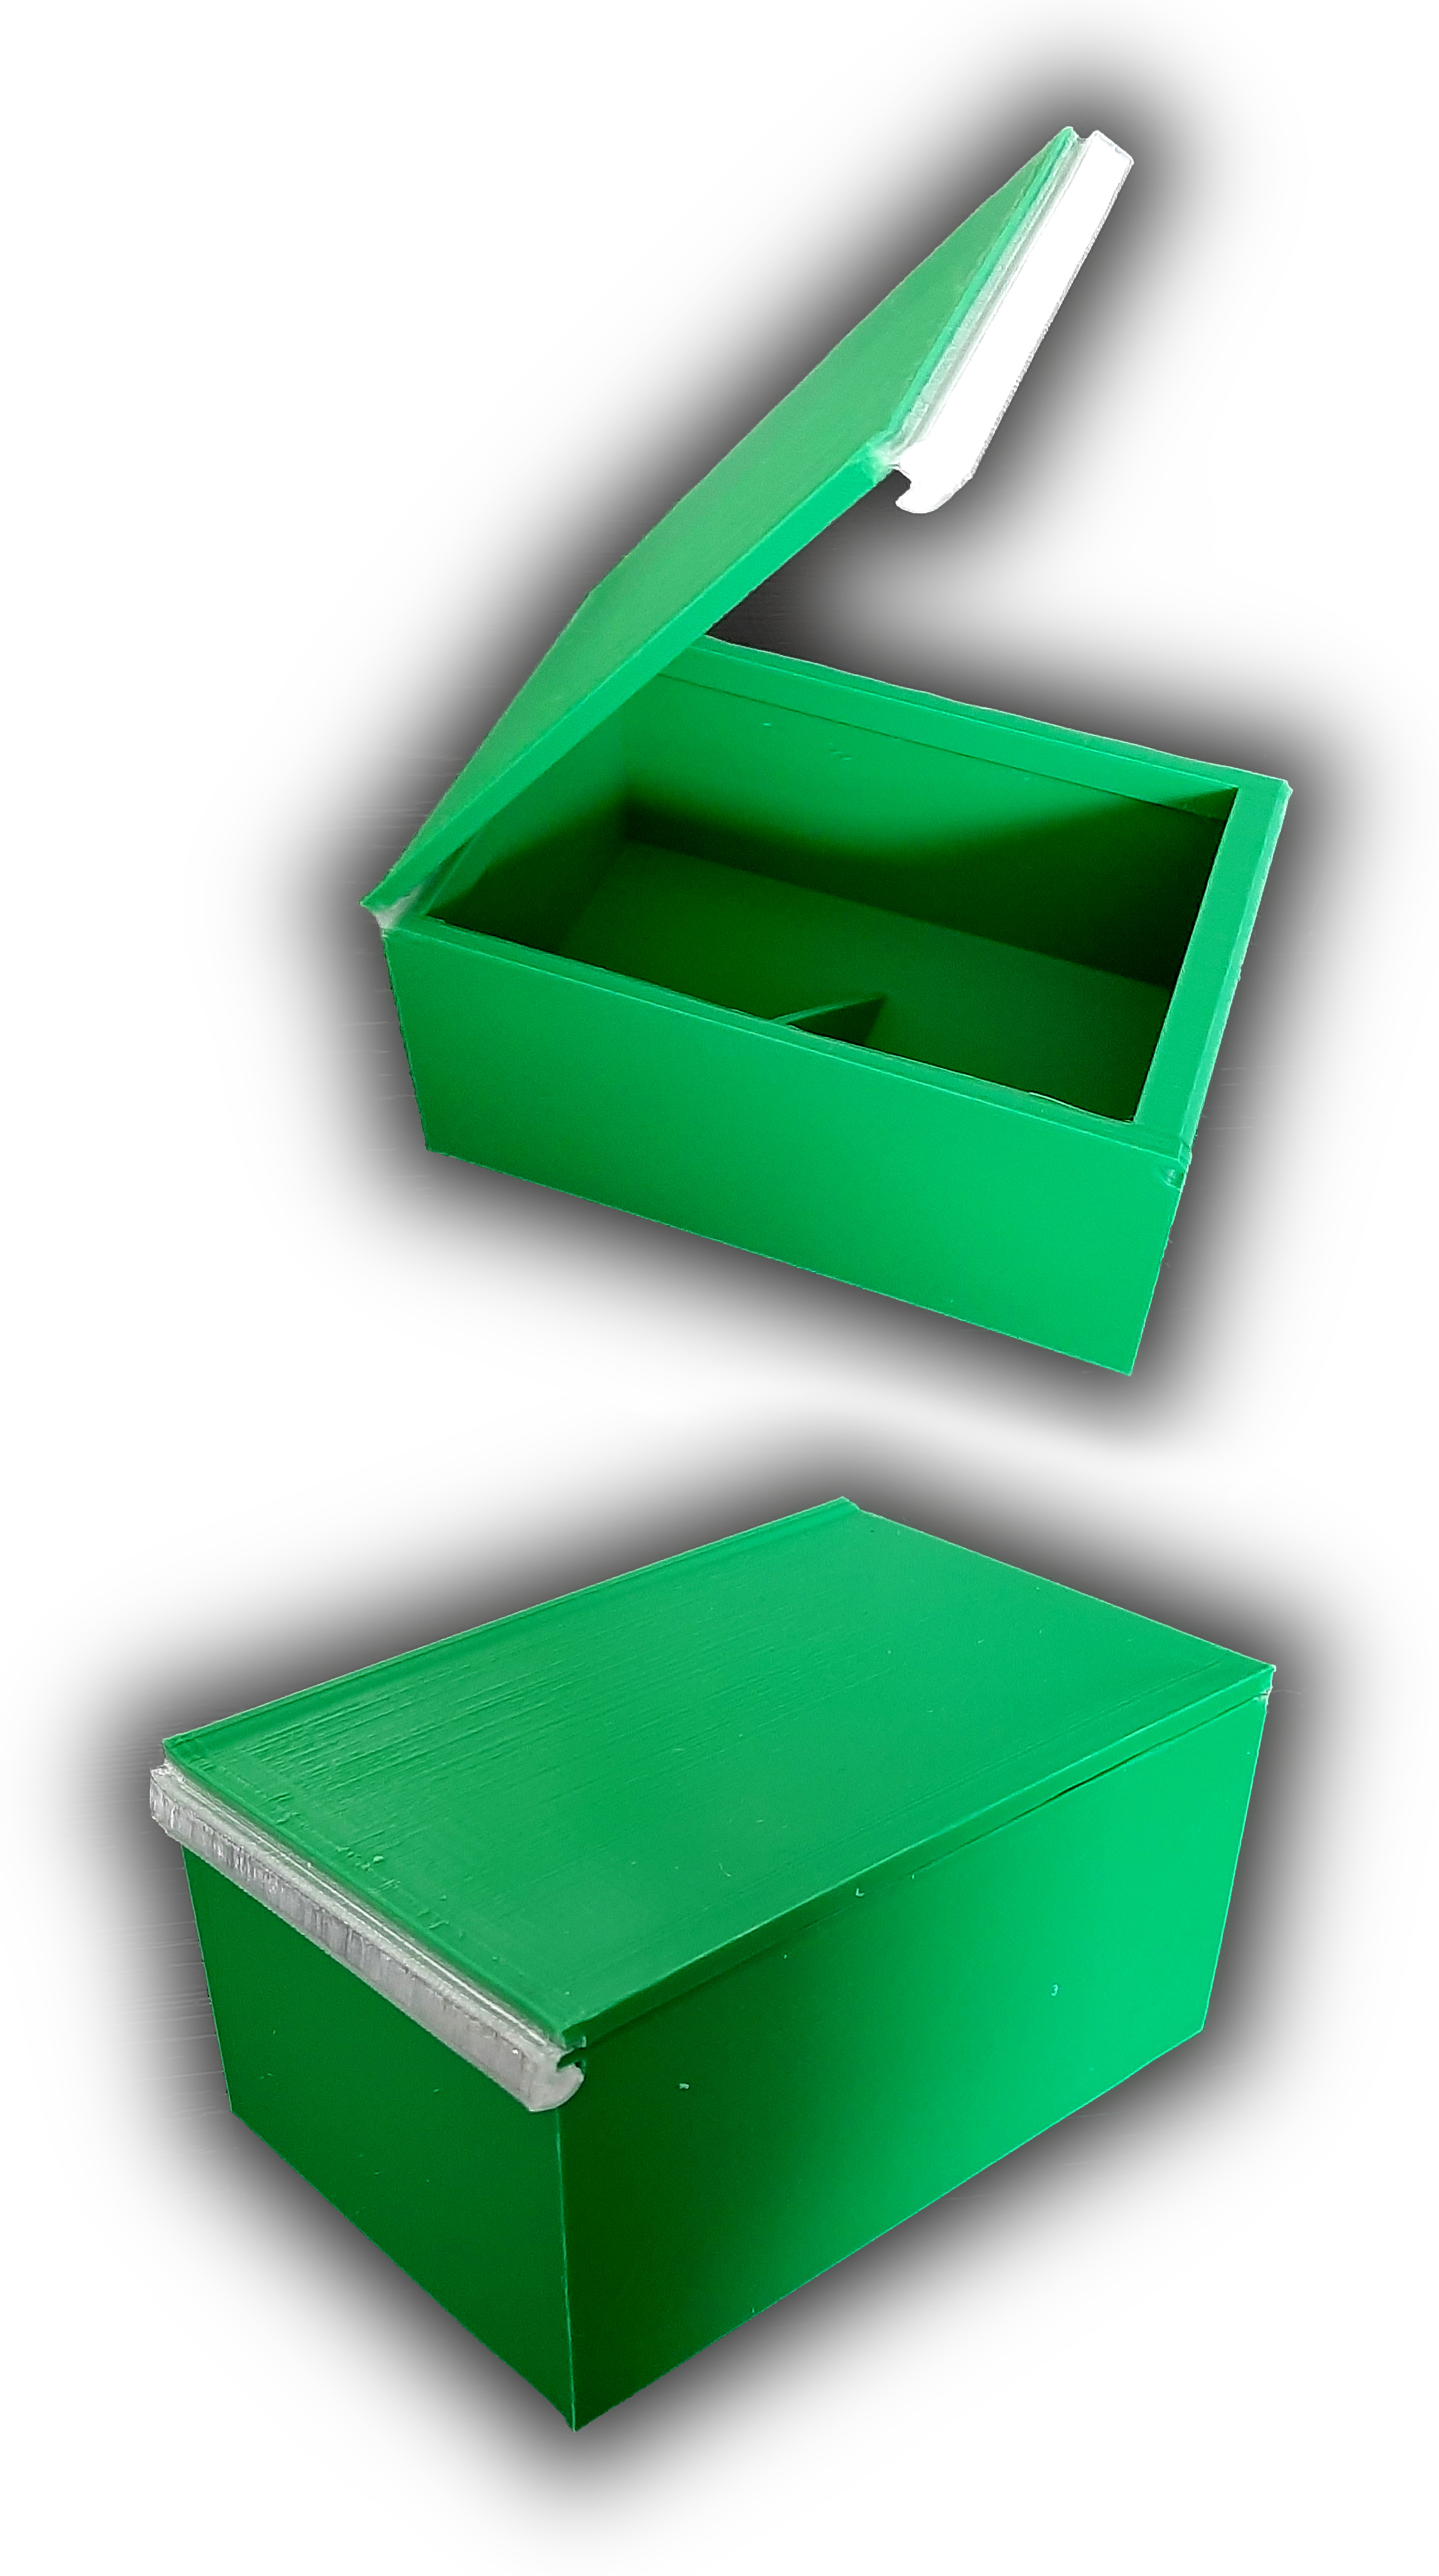
\includegraphics[height=\figheight]{sources/applications/storage_box.jpg}
		\caption{Storage box}
	\end{subfigure}
	\caption{Applications of interlocking structures.}
	\label{fig:applications}
\end{figure}




\subsection{Future work}
Future work might be aimed at loading scenarios different from tensile, different materials, different nozzle sizes and different layer heights.
It is specifically compelling to investigate the resilience of the interlocking structure against vertically applied loads.
Another interesting route is to optimize for an interface between two bodies which has a complex geometry and heterogeneous stress distribution.

In the light of sustainability and recycling one might select for specific failure modes, such as Z shear failure, which don't leave parts of the one material attached to the body of the other material after failure.

If the design constraint on the length of the transitional structure between the two material is released,
the manufacturing constraints are less relevant, which means that the geometry of the structure is less restricted.
The geometry of the microstructures could then be optimized for tailored mechanical properties.
In fact, such multi-material microstructures could be tailored for functionally graded materials.
With a relatively large geometry of the functionally graded multi-material lattice structure,
the IGIM lattice can again be used to ensure connectivity between the two materials,
while the meso-scale structure could be used to guarantee the functionally graded mechanical properties.
